% !TEX spellcheck = it-IT en-US
% !TEX encoding = UTF-8 Unicode
% !TEX root = main.tex

\documentclass[11pt,a4paper,twoside,openright,titlepage]{book}


\newcommand{\thesisTitle}{Thesis title}
\newcommand{\thesisAuthor}{Simone Porcu}	%author and title of the thesis - load before "init"
\usepackage[utf8]{inputenc}
\usepackage{movie15}
\usepackage[italian,english]{babel}
\usepackage{amsmath}
\usepackage{amsfonts}
\usepackage{amssymb}
\usepackage{amsbsy}

\usepackage[left=4cm,right=4cm,top=4.5cm,bottom=4cm]{geometry}
\usepackage{float}
\usepackage{color}
\usepackage[usenames,dvipsnames]{xcolor}
\usepackage{subcaption}

\usepackage[swapnames]{frontespizio}
\usepackage{emptypage}

\usepackage{url}

\usepackage{fancyhdr}
\usepackage{fancyvrb}\VerbatimFootnotes

\usepackage{csquotes}

\usepackage[
	pdftitle={\thesisTitle},
	pdfauthor={\thesisAuthor},
	pdfsubject={Master Thesis},
	%hidelinks,
	%linktocpage=true
	%backref=page			%enable back references
]{hyperref}

\usepackage{mdframed}


\usepackage[chapter]{minted}
\makeatletter	%minted fix for background%
\patchcmd{\minted@colorbg}{\noindent}{\medskip\noindent}{}{}
\apptocmd{\endminted@colorbg}{\par\medskip}{}{}
\makeatother

\usepackage{listings}


%\setminted{fontsize=\footnotesize}
\usemintedstyle{friendly}
%'default', 'pastie', 'perldoc', 'xcode', 'friendly', 'trac', 'vs', 'borland', 'igor', 'autumn'

%\usepackage{caption}
%\newenvironment{longlisting}{\captionsetup{type=listing}}{}

\usepackage[
	backend=bibtexu,
	bibencoding=utf8,
	backref=true,
	urldate=iso8601,
	date=iso8601
	]{biblatex}


\usepackage[nottoc,numbib]{tocbibind}		% include "List of ..." into the ToC



%% from scaffolding
\usepackage{titlesec}
\usepackage{stmaryrd}
%\usepackage{graphicx}
\usepackage{marvosym}


\usepackage{pdfsync}
\usepackage{wasysym}
%\usepackage{chemarr}

\usepackage[official]{eurosym} % Euro symbol (opts: official or gen)

\usepackage{alltt} % for math mode within verbatim

% \usepackage{enumerate} % Fancy enumeration styles

\usepackage{fixltx2e} % Text mode subscript and superscript
\usepackage{xspace} % Smart spaces after commands

\usepackage{nicefrac}
\usepackage{thmtools, thm-restate, thm-autoref}  % Advanced theorem handling

%\graphicspath{{figures/}} \DeclareGraphicsExtensions{.pdf,.jpg}
%\usepackage[center]{subfigure}
%\renewcommand{\subfigcapskip}{3pt}

% For custom alignment in itemize and description
\usepackage[inline,shortlabels]{enumitem} 
\newlist{inlinelist}{enumerate*}{1}
\setlist*[inlinelist,1]{%
	label=(\roman*),
}

%\usepackage{appendix} % conflict with LNCS style


\usepackage{cleveref}


\usepackage{fixltx2e} % Text mode subscript and superscript
\usepackage{xspace}   % Smart spaces after commands
\usepackage{xifthen}  % Extended conditional commands

%\usepackage{tikz} % for graph of module importation --- load LAST!

\usepackage{ifthen}

\usepackage[toc,page]{appendix}
			%packages declaration
%
% ABSTRACT
%
\newenvironment{abstract}%
{
	\cleardoublepage%
	%\thispagestyle{empty}%
	\thispagestyle{plain}%
	\null 
	\vfill
	\begin{center}%S
	\bfseries \abstractname 
	\end{center}
}%
{
	\vfill
	\null
}
			%commands and environment definition

% add bibliography databases
\bibliography{bib/main.bib}

\begin{document}

% ================================================================
% PARTE INIZIALE
% ================================================================
\frontmatter

\begin{frontespizio}
\Preambolo{\renewcommand{\frontsmallfont}[1]{\small}}	%rimuove la scritta 'Matricola'
\Preambolo{}
\Logo[3cm]{img/logo-unica.pdf}
\Universita{Cagliari}
\Facolta{Scienze}
\Corso[Laurea Magistrale]{Informatica}
\Titoletto{}
\Titolo{White blood cells segmentation using Vector Field Convolution}
\Candidato[]{Simone Porcu}
\Relatore{Prof. Cecilia Di Ruberto}
\Annoaccademico{2016-2017}

\Rientro{1cm}
\Margini{2cm}{2.5cm}{2cm}{2cm}
\Punteggiatura{}
\end{frontespizio}


\cleardoublepage
\null
\vspace{\stretch{1}}
\thispagestyle{empty}
\begin{flushright}
\textit{To my family}
\end{flushright}
\vspace{\stretch{2}}
\null
\chapter*{Abstract}

The analysis, counting and classification of white blood cells in automatic way is also an unresolved issue. This automation could be very helpful in medical field, to recognize the kind of pathology that affect a patient. Now the recognize method is completely handmade. In every medical center exist an expert that work hardly to analyse, count and classify the white blood cells in the peripheral blood.

\bigskip

His work is divide in three steps and everyone of these steps is very long. in particular we have to focused on a particular issue that could affect the optimal result of the work. The analyser after many hours of work due to the fatigue of sight may not see it as well as before and maybe not see certain particulars that affect cells that could completely change the patient's diagnosis.

\bigskip

Our propose is to create a system that in automatic way is able to do every single step of the blood expert work. We want to do this to decrease the time and increase the efficiency of the process.

\bigskip

Our solution is use a vector field VFC to describe cells edges, without using the active contour model. We choose this approach because we concentrate our work on the segmentation of the white blood cell in overlap position.

\bigskip

At the end we defined a system that is able to recognise the leukocytes by the other cells of the peripheral blood and divide the leukocytes in overlap with another one. Then in conclusion we trying to construct a method able to divide the main unresolved issue of the leukocytes segmentation.




\cleardoublepage
\setcounter{page}{1}
\pagenumbering{Roman}

\cleardoublepage
\setcounter{page}{1}
\pagenumbering{roman}
\tableofcontents

% ================================================================
% CORPO CENTRALE
% ================================================================
\mainmatter

\chapter*{Introduction}
\addcontentsline{toc}{chapter}{Introduction}
This project has been developed under the supervision of Prof. Cecilia Di Ruberto and PhD students Andrea Loddo and Lorenzo Putzu.

\bigskip


Blood is a body fluid deliver. It's contains an transport many of the nutrients substances that the man and the other animals use to live. That we call blood is principally a fluid divided in two elements: blood cells and blood plasma. Normally an individual has around 5 Litre of blood. The plasma blood constitutes the 55\% of the total fluid. it is mostly water(92\% by volume) and contains proteins, glucose, mineral ions, hormones and blood cells themselves.\cite{website:wiki} Mainly the cells are red blood cells and white blood cells(WBCs). In this dissertation we going to focus on WBC especially we will study the shape of these last.
White blood cells, also called leukocytes , are the cells with the task of controlling the body against both infectious disease and foreign invaders. All leukocytes have a nuclei that distinguishes them by other blood cells, in particular red blood cells and platelets. The generic term leukocytes includes very different cells population: neutrophil, granulocytes, basophilic granulocytes and eosinophilic granulocytes. This set of three categories is defined as   polymorphonucleated granulocytes. The other set that includes monocytes and lymphocytes is defined agranulocytes mononuclear. In a nutshell leukocytes are dived in these two sets by the nuclei shape.\ref{fig:kindLeuko}
\begin{figure}
	\begin{center}
		\centering
		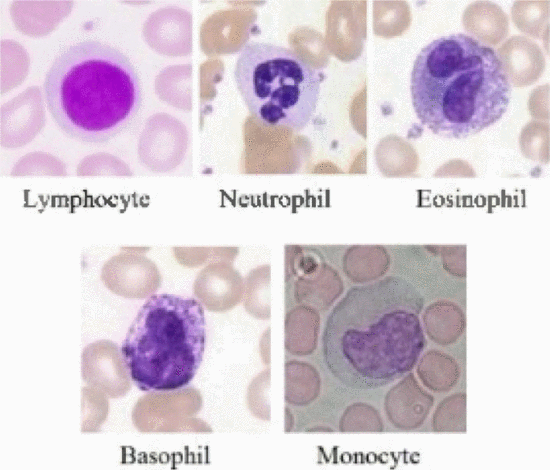
\includegraphics[scale=0.5]{img/leuko.png}
		\caption{Example of the different kind of leukocytes\cite{ann17}}
		\label{fig:kindLeuko}
	\end{center}
\end{figure}

\section*{White blood cells segmentation}
Segment an image means divide an image in regions of interest. It's used to obtain a more compact image used to extract objects or to analyse an image. More precisely, image segmentation is the process of assigning a label to every pixel in an image such that pixels with the same label share certain visual characteristics. In this case the main feature is to find edges and white blood cells nuclei. At a first look seems a banal problem, because the we think that every single cell is strongly separated by the others, but obviously it is the best case that we can find. Commonly the microscope photos that we analyse contains noise and in particular the leukocytes overlaps both others leukocytes and red blood cells. For these reasons segment leukocytes is still an unresolved problem. As explain above there are 2 class of leukocytes that are dissimilar by the nuclei shape. this is an high problem because if the solution to find all the white blood cells was based on the search of circular shapes, it's trivial that it will be impossible to recognize a granulocytic from a monocyte.


\bigskip


There are a lot of heuristics and approaches that try to divide white blood cells. This dissertation proposes a new approach of pure segmentation using the Vector Field Convolution, in particular tries to find a division between the overlaps between the cells. The used dataset is ALL-IDB dataset, a public dataset created by the University of Milan. It contains microscopic images of blood samples, specifically designed for the evaluation and the comparison of algorithms for segmentation and image classification.


\bigskip 


We choose this vector field because the common practice to extract the features by the images utilizes thresholds, but what happens if the image has a low definition and all the cells are in overlap with their? Using that field to describe the image is possible to transcend by the shape of the features and focus themselves on the points that have a non-uniform virtual field. This technique then considers only the points that describe the edges of the white blood cells. After the image elaboration the result is an image that contains only leukocytes and when it is necessary dividing every kind of cells. With this result we can label every cell without human work.


\bigskip


The first step of the algorithm pre-processes the image in order to overcome the non-linearity  of colour distribution inside the image. The literature says that we can overtake this problem using the mean-shift model. The second step applies the Vector Field Convolution on the edge image obtained by the first step, in order to obtain an intensity image of the cells. The third step focuses is work on the extraction of the angle image in order to obtain the direction of each pixel and to apply to it the Energy function. The fourth step applies the median filtering to the energy image and the angle image and puts them in overlay in order to apply the skeleton function after an opening of the closing. After this step we obtain, joining the skeleton image with the leukocytes image and the Energy image, the first result: the segmentation of the cells and in particular also the segmentation of the cells in overlap.
The fifth step counts the cells.

\part{Background}

\chapter{Overview about vector fields and segmentation techniques}
\section{The vector field}
What is a vector field? A Vector field is an assignment of a vector to each point in a subset of space. This assignment is the value that will give an orientation to the row that will describe our image.
\begin{figure}
	\centering
	\begin{subfigure}[b]{0.5\textwidth}
        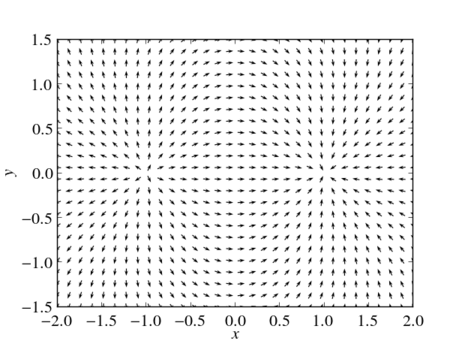
\includegraphics[width=\textwidth]{img/fieldex.png}
        \caption{ }
        \label{fig:field}
    \end{subfigure}
    \begin{subfigure}[b]{0.5\textwidth}
		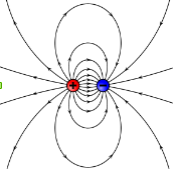
\includegraphics[width=\textwidth]{img/dipole.png}
		\caption{ }
		\label{fig:dipole}
	\end{subfigure}
	\caption{(a) Dipole electric field, (b) Electric dipole}
	\label{fig:fielddipole}
\end{figure}
The figure \ref{fig:fielddipole} represent a vector field flow of an electric dipole \ref{fig:dipole} in the $x-y-plane$ with $r+=(-1,0,0) and r-=(1,0,0)$. All vectors are normalized to the unity. Thus, the plot visualizes the direction of the electric dipole field, but not the field strength. In the negative zone part of the dipole it is possible to see that rows of the vector field tries to enter the plane and at the opposite side it’s possible to see the exact opposite, that shows the rows exit from the plane. This translates into a flow of rows that is possible to applicate to describe the leukocyte's edges.

Active contours, also called snakes, are curves that move inside the image following the energy of the field. There are two kinds of forces, one internal and anther external. Combining these two it's possible to create a curve that follows constraints gives by the forces. The  internal  and  external  forces  are  defined  so  that  the  snake  will conform to an object boundary or other desired features within an image. Snakes are widely used  in  many  applications,  including  edge  detection,  shape  modelling and segmentation. There  are  two  general  types  of  active  contour  models  in  the literature  today:  parametric active contours and geometric active contours. Typically,  the  curves  are  drawn  toward  the edges  by  potential  forces,  which  are  defined  to  be  the  negative  gradient  of  a  potential function.  Additional  forces,  such  as  pressure  forces,  together  with  the  potential  forces comprise the external forces. There are also internal forces designed to hold the curve together and to keep it from bending too  much.  There  are  two  levels  difficulties  with  active  contour  algorithms.  First,  the  initial contour must be close to the true boundary or else it will likely converge to the wrong result. The second problem is that active contours have difficulties progressing into concave  boundary  regions.  Although  many  methods  such  as  multi resolution  methods, pressure forces, distance potential forces, control points, and using solenoidal external fields have been proposed they either solve one problem or solve both but creating new difficulties. For  example,  multi resolution  methods  have  addressed  the  issue  of  initialization,  but specifying  how  the  snake  should  move  across  different  resolutions  remains  problematic. Another example is that of pressure forces, which can push an active contour into boundary concavities, but cannot be too strong or “weak” edges will be overwhelmed. But how works a snake if the objects to segment are overlapped? Snakes are able to find all the external edges of the object but in this case the edge can be consider an internal part of the object. With the active contours is impossible segment the overlapped cells because the snake cannot enter inside the cell region. For these reason we have used our virtual field following another lecture key.

\section{An overview of Image Segmentation methods}
when we talking about segmentation we introduce a technique for partitioning the image into subregions. Below are described the most five famous techniques to develop an image segmentation:
\begin{enumerate}
	\item threshold-based;
	\item histogram-based;
	\item region-based;
	\item edge detection;
	\item watershed transformation
\end{enumerate}
\subsection{threshold-based techniques}
Thresholding is the simplest segmentation method. The pixels are partitioned depending on their intensity value generally used with gray scale images $f(x,y)$. When the threshold is apply on gray scale images the final target is separate the foreground by the background. The first one contains only the element of interest and the second one contains all the rest of the image. The global threshold value T is the 'breaking point' of the image. After an analysis of the image, the value T is used to understand if, taking in account each pixel of the image,each one it belongs to the foreground $f(x, y) > T$ or to the background $f(x, y) < T$ . used to understand if, taking in analysis each pixel of the image, it's below to the foreground $f(x, y) > T$ or to the background$f(x, y) < T$.\cite{Threshold}

\subsection{Histogram-based techniques}
An important class of point operations is based upon the manipulation of an image histogram or a region histogram. It uses the histogram to select the gray levels for grouping pixels into regions. The image is composed by the foreground and the background. Generally the background occupies most of the image and for this reason it's gray level will be a large peak in the histogram. The object of the image as opposed to the background is a smaller peak in the histogram. Then we can choose a threshold point in the valley between the two peaks and threshold the image.

\subsubsection{Region-based techniques}
Differently from the other two techniques described before the region-based segmentation is a technique for determining the region directly.Initially set of point of interest
are created. Starting from these points other regions grow up if neighbouring pixels have
similar properties as that of point of interest. In region splitting and merging, an image
is subdivided into different regions and then either merged and split. As first step the image is split into four disjoint quadrants, then merges any adjacent regions, which satisfy the imposed constraints. Like a loop we repeat splitting of regions and merging till no further merging or splitting is
possible. Image regions are implemented with the help of quad trees.
The basic formulation is:$\\
(a){\text{ }}\bigcup \nolimits _{{i=1}}^{{n}}{R_{{i}}=R.}\\
(b){\text{ }}R_{{i}}{\text{ is a connected region}},{\text{ i}}={\text{1}},{\text{ 2}},{\text{ }}...,{\text{n}}\\
(c){\text{ }}R_{{i}}\bigcap R_{{j}}=\varnothing\\
(d){\text{ }}P(R_{{i}})=TRUE{\text{ for }}i=1,2,...,n.\\
(e){\text{ }}P(R_{{i}}\bigcup R_{{j}})=FALSE{\text{ for any adjacent region }}R_{{i}}{\text{ and }}R_{{j}}\\
$
$P(R_{{i}})$ is a logical predicate defined over the points in set $R_{i}$ and $\varnothing$  is the null set.
(a) means that the segmentation must be complete; that is, every pixel must be in a region.
(b) requires that points in a region must be connected in some predefined sense.
(c) indicates that the regions must be disjoint.
(d) deals with the properties that must be satisfied by the pixels in a segmented region. For example, $P(R_{{i}})={\text{TRUE}}$ if all pixels in $R_{i}$ have the same gray-scale.
(e) indicates that region $R_{i}$ and $R_{{j}}$ are different in the sense of predicate $P$.\cite{website:region_g}

\subsection{Edge detection technique}
Edge detection includes a variety of mathematical methods that aim at identifying points in a digital image at which the image brightness changes sharply or, more formally, has discontinuities. The points at which image brightness changes sharply are typically organized into a set of curved line segments termed edges. The same problem of finding discontinuities in one-dimensional signals is known as step detection and the problem of finding signal discontinuities over time is known as change detection. Edge detection is a fundamental tool in image processing, machine vision and computer vision, particularly in the areas of feature detection and feature extraction.\cite{edge} Is possibe to divide Edges in two different set: intensity edges and texture edges. The first one includes steps and roofs. The Texture edges set include all the regions that are invariant to the luminance conditions. Then to obtain a continuous edge is necessary a function of edge linking. Below there are the most famous edge detection algorithms: Sobel, Prewitt, log, zero-cross, Roberts, Canny.

\subsection{Watershed technique}
This function considers the magnitude of the image like a topografic surface. In proximity of the watershed lines the pixels have an high magnitude intensity. The water is put inside the regions enclosed by the watershed lines. As is possible to understand from these lines we are talking about a global local minimum. We said it because for each region (local) we find the global minimum and we fill it with the water.

\bigskip

Next chapter illustrates, in detail, how we use the Mean Shift segmentation technique and the use of it's result with the VFC.
\part{About Mean Shift}
\chapter{Mean shift}
The mean shift procedure was originally presented in 1975 by Fukunaga and Hostetler. It is a no-parametric method for locating the modes of a density function in  discrete data sampled. It is an iterative method that start with an initial estimate $x$.
\section{Mean shift kernel function}
Given a kernel function $K(x_{i}-x)$, as the function that determines the weight nearby points to re-estimate the mean. The kernel function has to respect the following constraints:
\begin{equation}
\int R^{d} \,\phi({x})=1 
\end{equation}
\begin{equation}
\phi ({x}) \leq 0
\end{equation}
The literature talk about some different kernel definitions, but typically to -mean shift use the Gaussian kernel or Epanechnikov kernel, respectively explained below:
\begin{equation}
\phi({x}) = e^{-\frac{x^{2}}{2\sigma^{2}}}
\end{equation}
\begin{equation}
K(x)={\begin{cases}\frac{3}{4}(1-x^{2})&{\text{if}}\ |x|\leq 1 \\0&{\text{else}}\  \\\end{cases}}
\end{equation}

\bigskip

Known as KDE, kernel density estimation, in statistics is consider a non-parametric way to estimate the probability density function of a random variable. KDE is a data smoothing problem where inferences about the population are made based on a finite data sample. when we work in the field of signal processing and econometrics it is termed the Parzen-Rosenblatt window method. 

\bigskip

Given an unknown density $f$ a distribution $X$, we want to estimate the shape of this function $f$. Its kernel density estimator is 
\begin{equation}
{{\hat {f}}_{h}(x)={\frac {1}{n}}\sum _{i=1}^{n}K_{h}(x-x_{i})={\frac {1}{nh}}\sum _{i=1}^{n}K{\Big (}{\frac {x-x_{i}}{h}}{\Big )}}
\end{equation} 
where the kernel $K(x)$ is a scalar function.

\section{Mean shift definition}
Define a d-variate kernel function $K(y)$ to be a search window; if it is symmetric:
\begin{equation}
K(y)= ck(\|y\|^{2})
\end{equation}
where $c$ is the normalization constant, $k(s)$ is a symmetric univariate kernel which that it is the profile of $K(y)$ if $s \geq 0$ and y is the center location of the search window. Calculating the ocation of the centroid of the search window we obtain a vector of the differences between the local mean and the centre of the window
\begin{equation}
m_{k}{(x)}= y_{centroid} - y
\end{equation} 
Defined $\xi$ as an arbitrary small value, indicating a threshold, if
\begin{equation}
\|m_{k}(y)\|^2 \geq \xi     
\end{equation}
As we said previously this is an iterative algorithm, then the search window can be moved iteratively, because it means that it has not find the convergence. The convergence is simply the value in which we can stop computing the mean shift value. Now is possible to define the other centre of the search window and start again the process.

\bigskip

In order to use this function the user has to choose three input parameters:
\begin{enumerate}
\item $h_{s}$ . Spatial bandwidth value in which the Mean Shift will be computed. It indicates the maximum radius within the pixels are considered for the computation of the Mean Shift value;

\item $h_{r}$  . Colour bandwidth value. It indicates the maximum colour difference between
actual pixel value and the pixel taken for the computation. If the difference is greater than $h_{r}$ , the pixel will not be considered for the computation of new value;

\item $th$. Threshold value. It represents the parameter $\xi$. When this value is reached, the algorithm terminates.
\end{enumerate}
\part{About Vector Field Convolution}
\chapter{Vector field convolution}
The vector field convolution is a snake external force created by Bing Li and S.T. Acton.

\bigskip

Convolving a vector field with the edge of the map derived from the image you get an external force, the VFC. Active contours using the VFC external force are called VFC snakes. Like the GVF snakes instead of being formulated using the standard energy minimization framework, VFC snakes are constructed from a state of equilibrium between the forces. The VFC snakes besides having a wide capture range and the ability to capture the concavities, are better resistant to noise image, have the ability to adapt the force field and reduce drastically the computational cost.
Before to explain the VFC it is right to explain the vector field kernel
\begin{equation}
 k ( x,y ) =m(x,y)n(x,y)
\end{equation}
where n is the unit vector that points to the origin of the kernel	
\begin{equation}
n ( x,y ) = [\frac{-x}{r} , \frac{-y}{r} ]
\end{equation}
and m is the magnitude of the vector . The authors of the VFC implemented two kinds of magnitude. If we consider the origin as the point of interest, this vector field kernel has the desirable property that a free particle placed in the field is able to move to the point of interest. The external force that works in the VFC is defined in this way:
\begin{equation}
{f} _{vfc} ( x,y ) = {u} _{vfc} ( x,y ) , {v} _{vfc} (x,y)
\end{equation}
Since the map of the edge is non-negative and is wider near the edges of the image, the edges act to a greater extent on the VFC than homogeneous regions. Therefore, the free particles of homogeneous regions will be attracted to the edges. If we present the vector field kernel using a complex-valued range, the VFC is just the filtering result of the edge map, which does not depend on the origin of the kernel. The VFC field highly depends on the magnitude of the vector field kernel . The field VFC has the magnitude directly proportional to the vector field kernel (x, y). Knowing that the figure of interest has less influence on the particles away from it, the magnitude must be expressed as a positive function decreasing with respect to the distance of the origin. Below we propose two types of magnitude functions, given as
\begin{equation}
{m} _{1} ( x,y ) =(r+\epsilon) ^{-\gamma}
\end{equation}
\begin{equation}
{m} _{2} ( x,y ) =exp(-r^{2}\, \zeta ^{2})
\end{equation}
where $\gamma$ and $\zeta$ are positive parameters to control the decrease, $\epsilon$ is a small positive constant to prevent division by zero at the origin. ${m} _{1} ( x,y )$ is inspired by Newton’s law  of universal gravitation in physics. Furthermore, the pixels in the edge map can be considered as objects of mass proportional to the strength of the edges and the field VFC would be the gravitational field generated by all objects. The influence of the figure of interest increases as $\gamma$ decreases. In practice $\gamma$ usually ranges from 1.5 to 3 for most images. ${m} _{2} ( x,y )$ is a Gaussian shape function, where $\zeta$ can be viewed as the standard deviation. The influence of the figure of interest increases as $\zeta$ increases. In general, the influence of the figure of interest should be increased (decrease or increase) as the signal-to-noise ratio is decreased.\cite{VFC}

\part{A parallel way of using VFC without active contours}
\chapter{The implementation}
For the implementation we followed the approach shows in the figure \ref{fig:diag}
\begin{figure}
	\begin{center}
		\centering
		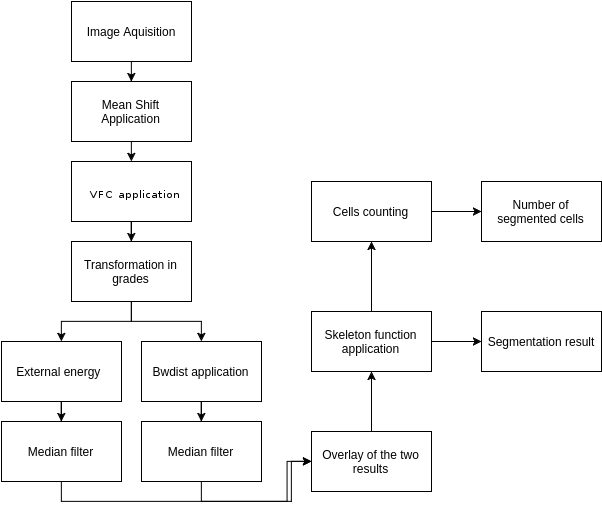
\includegraphics[scale=0.5]{img/diag.png}
		\caption{Method diagram representation}
		\label{fig:diag}
	\end{center}
\end{figure}

\section{New kind approach to segment leukocytes}
As we can see in literature, the main approach used to resolve the overlap problem is using the watershed transform. Here\ref{fig:overlap} there is an example of the watershed transform. Takes in input the image of the two overlapped circles, we calculate the distance transform, or in other words we calculate the Euclidean distance transform of the binary image BW. For each pixel in BW, the distance transform assigns a number that is the distance between that pixel and the nearest non-zero pixel of BW\ref{fig:overlaptransf}.Giving the distance transform result to the watershed algorithm we obtain a division between circles because the watershed transform finds "catchment basins" or "watershed ridge lines" in an image by treating it as a surface where light pixels represent high elevations and dark pixels represent low elevations.\ref{fig:overlapwater}
\begin{figure}[htbp]
    \centering
    \begin{subfigure}[b]{0.5\textwidth}
        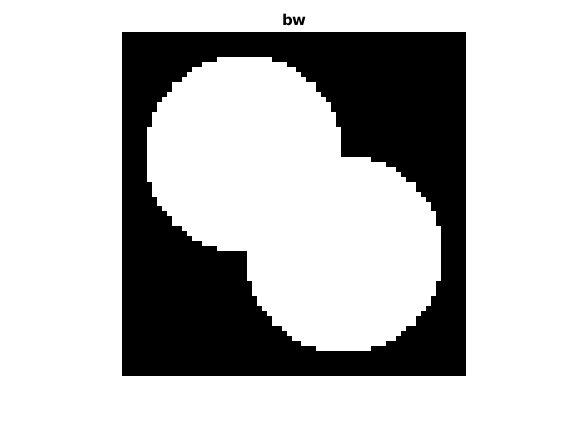
\includegraphics[width=\textwidth]{img/circlesEx.png}
        \caption{ }
        \label{fig:overlap}
    \end{subfigure}
     \quad
      %(or a blank line to force the subfigure onto a new line)
    \begin{subfigure}[b]{0.5\textwidth}
        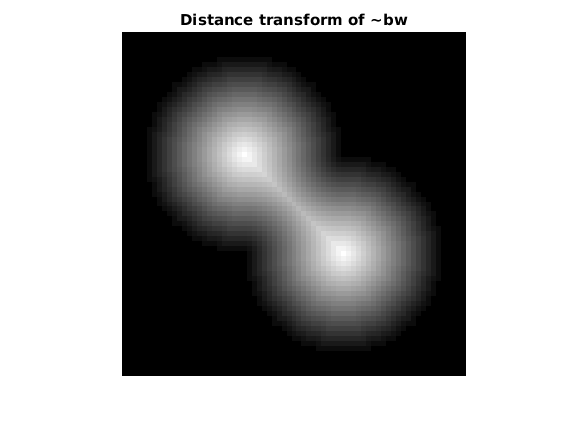
\includegraphics[width=\textwidth]{img/distancerTransform.png}
        \caption{ }
        \label{fig:overlaptransf}
    \end{subfigure}
    \quad
    \begin{subfigure}[b]{0.5\textwidth}
        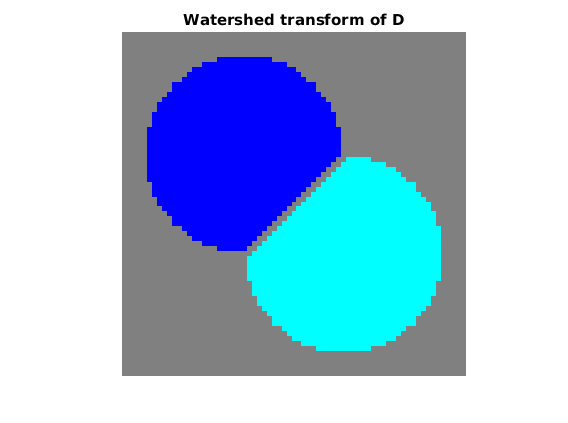
\includegraphics[width=\textwidth]{img/watershedEx.png}
        \caption{ }
        \label{fig:overlapwater}
    \end{subfigure}
    \caption{(a) Example of two circle in overlap, (b) Distance transform, (c) Watershed result}\label{fig:stepswater}
\end{figure}
This is an ideal case to analyse. But when we work with the overlapping between cells the result of the division by Watershed transform is not optimal like the example \ref{fig:stepswater}. Probably the cause derived from the low definition of the figures and especially the shape of the cells. Here there is an example of what happened when we try to divide 3 cells in overlap\ref{fig:exOnImage7}.
\begin{figure}
	\centering
	\begin{subfigure}[b]{0.5\textwidth}
        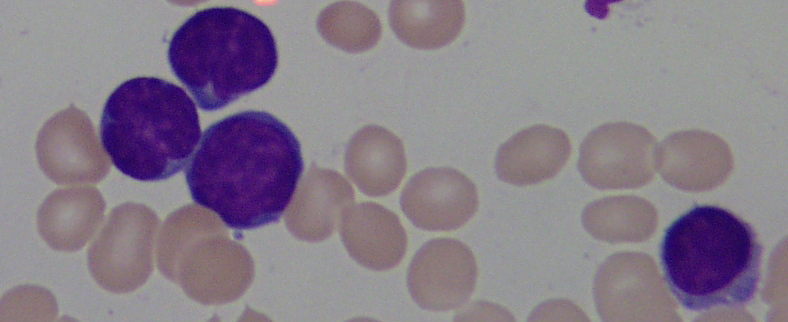
\includegraphics[width=\textwidth]{img/Im007_1_crop.png}
        \caption{ }
        \label{fig:origimage}
    \end{subfigure}
    \begin{subfigure}[b]{0.5\textwidth}
		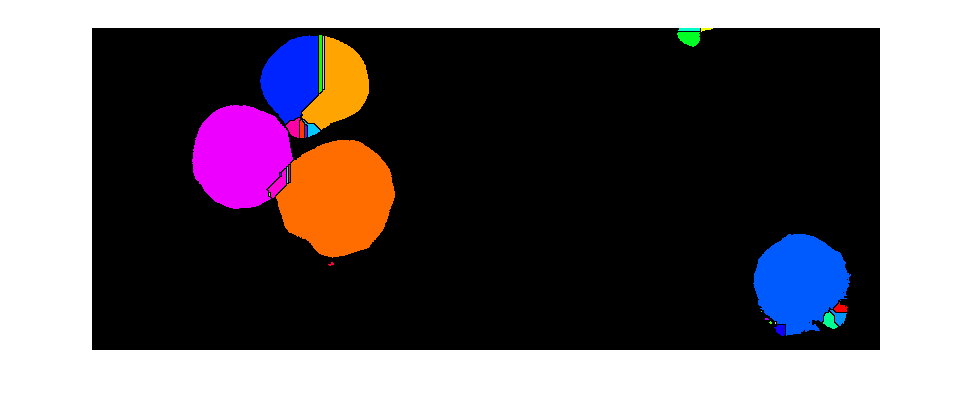
\includegraphics[width=\textwidth]{img/waterTrRes.png}
		\caption{ }
		\label{fig:watershedoncells}
	\end{subfigure}
	\caption{(a) Original leukocytes image, (b) Watershed transform applied to three cells in overlap}
	\label{fig:exOnImage7}
\end{figure}
As is possible to see, this method produce a no-realistic separation of the cells. For this reason we study a different method that in automatic way produce a realistic division of the cells. Starting from the resulting image after the application of the mean shift algorithm, we based our implementation using principally the output of the VFC field, the image relative to the External energy of the image to describe the edges, the median filter and the skeleton method.
\section{ALL-IDB blood cell dataset}
The images of the dataset have been captured with an optical laboratory microscope coupled with
a Canon PowerShot G5 camera. All images are in JPG format with 24-bit colour depth. The first 33
have $1712*1368$ resolution, the remaining have $2592*1944$ resolution. The images are taken with
different magnifications of the microscope ranging from 300 to 500 which brings the colour
differences that we managed grouping the images with same brightness characteristics together. The
ALL-IDB database has two distinct folders (ALL-IDB1 and ALL-IDB2).

\bigskip

The table \ref{tableidb} shows a little description about the images.
\begin{table}
\centering
\begin{tabular}{|c|c|c|}
\hline 
Characteristic & ALL-IDB1 & ALL-IDB2 \\ 
\hline 
Images & 109 & 260 \\ 
\hline 
Max resolution & 2592x1944 & 257x257 \\ 
\hline 
Elements & 39000 & 260 \\ 
\hline 
Candidate Lymphoblasts & 510 & 130 \\ 
\hline 
\end{tabular} 
\caption{Characteristics of the dataset. Images acquisition has been performed with a Canon PowerShot G5. Magnification of microscope goes from 300 to 500. The image format of the ALL- IDB1 folder images is JPG, ALL-IDB2 images have TIF format. The colour is 24 bit depth.}
\label{tableidb}
\end{table}
The IDB1 set can be used both for testing segmentation capability of algorithms, as well as the classification systems and image preprocessing methods. This dataset is composed of 108 images collected during September, 2005. It contains about 39000 blood elements, where the lymphocytes has been labelled by expert oncologists.\cite{website:IDB}
The IDB2 set has been designed for testing the performances of classification systems. The ALL-IDB2 version 1.0 is a collection of cropped area of interest of normal and blast cells that belongs to the ALL-IDB1 dataset. ALL-IDB2 images have similar gray level properties to the images of the ALL-IDB1, except the image dimensions.\cite{website:IDB}
For our work we consider only normal leukocytes and we focused principally on the images where is present an overlap between the white blood cells.

\section{Mean shift application}
In order to resolve the illumination problems and to obtain a good visualization of the Wright-Giemsa stain cells we use the mean shift function. To obtain an acceptable result should be necessary, but using the bandwith parameters and the threshold parameter of the mean shift function we can obtain the same result. For our work we used $h_{s}$ (bandwith of the spatial kernel) = 4, $h_{r}$ (colour bandwith) = 4 and the threshold $th$ = 0.25. The result changing these parameters is not so significant in order to obtain a good final result, then is preferable use an image with a little bit definition but obtained in a very short time (2 seconds).

\section{The VFC result}
The VFC uses the two components of the external force ${u} _{vfc} ( x,y ) , {v} _{vfc} (x,y)$ to describe the field of the image and it's magnitude. Our purpose is find and image using these two components that describes all the leukocytes edges taking an accurate look on the edges in overlap. The first step then is extract the right component and the left component.
\begin{equation}
{u} _{vfc}=ExtF(x)/\sqrt{ExtF(x)^{2} + ExtF(y)^{2}}
\end{equation}
\begin{equation}
{u} _{vfc}=ExtF(y)/\sqrt{ExtF(x)^{2} + ExtF(y)^{2}}
\end{equation}
where ExtF is the External force of the field. Now we have only an intensity image, but to understand how the field moves in the space we have to transform these two component $ u$ and $ v $ in grades. It a mandatory do this step because we want to understand the direction of every pixel in the figure. Is possible convert the two components in degrees using the $atan2d$ function \ref{fig:angle}.
\begin{figure}
	\begin{center}
		\centering
		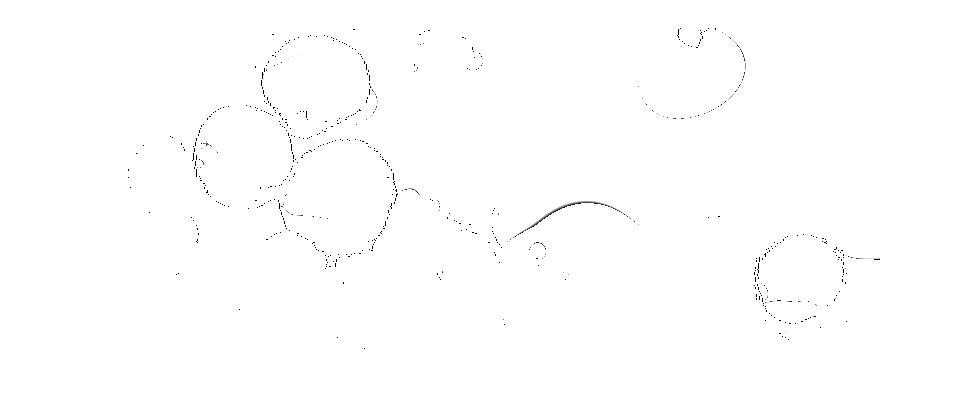
\includegraphics[scale=0.5]{img/angle.png}
		\caption{degrees image}
		\label{fig:angle}
	\end{center}
\end{figure}
In order to delete all the uniform part of the figure and put in exalt the edges we use a mediand filter using the function $ordfilt2$ searching the 18th element of the $5 * 5$ mask \ref{fig:Pmedangle}.
\begin{figure}
	\begin{center}
		\centering
		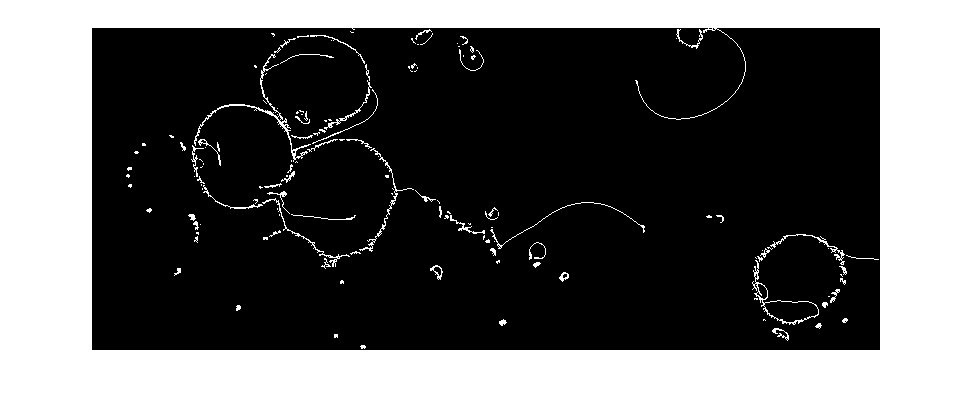
\includegraphics[scale=0.5]{img/PmedAngle.png}
		\caption{Median filter on degrees image}
		\label{fig:Pmedangle}
	\end{center}
\end{figure}
\section{External Energy}
As is possible to see in the result \ref{fig:angle}, there are a lot of points that are artefacts created by the field. For these reason we used the $bwdist$ function to assign a number that it is the distance between each pixel and the nearest no-zero pixel of the image. This trick is very useful because reduce the entropy of the image, focusing only on the shape of the leukocytes \ref{fig:bwdistangle}.
\begin{figure}
	\begin{center}
		\centering
		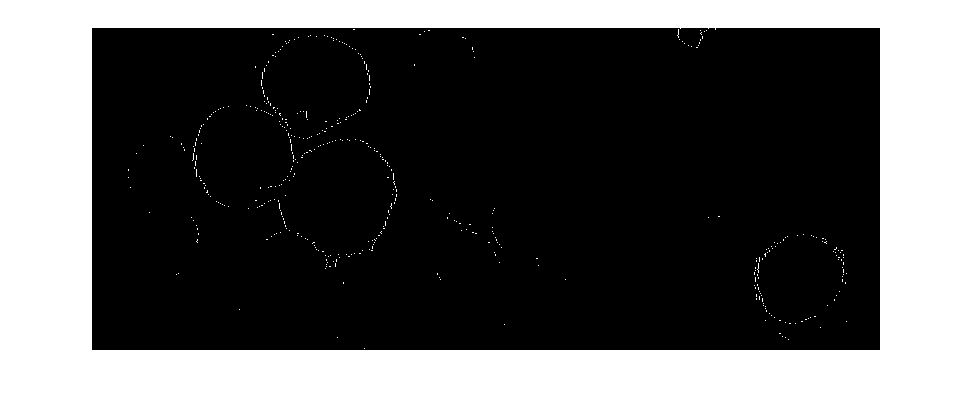
\includegraphics[scale=0.5]{img/bwdistAngle.png}
		\caption{bwdist applied on degrees image}
		\label{fig:bwdistangle}
	\end{center}
\end{figure}
But we have ever the same problem. in the image there are trace of the red blood cells, then we had to find a method to isolate only the leukocytes. We started using the external energy of the image. For an image $I(x,y)$ all the lines, edges and terminal points the general formulation of the Energy of the image is
\begin{equation}
 E_{image}=w_{line}E_{line} + w_{edge}E_{edge} + w_{term}E_{term}
\end{equation}
where $w_{line}, w_{edge}, w_{term}$ are weights of the features.

\subsection{Line functional}
The line functional or in other terms the intensity of the image is in a nutshell the attracted value of the dark lines to the light line. It's possible choose this attraction putting a positive or negative sign before the force that this attraction has to be.
\begin{equation}
	E_{{line}}=filter(I(x,y))
\end{equation}

\subsection{Edge functional}
The edge functional bases it's work on the image gradient.
\begin{equation}
E_{{edge}}=-\left|\nabla I(x,y)\right\vert ^{2}
\end{equation}
It's very useful because when we try to analyse the feature of the image, we work with maxims and minims. with this formula we can avoid the local minima that are not object of interest. The energy functional using scale space continuation is
\begin{equation}
E_{edge}=-\left|G_{\sigma }*\nabla ^{2}I\right\vert ^{2}
\end{equation}

where $ G_{\sigma } $ is a Gaussian with standard deviation $ \sigma $.

\subsection{Termination functional}
The curvature of the lines in a image is utilized to detect corners and terminations. Put 
\begin{equation}
C(x,y)=G_{{\sigma }}*I(x,y)
\end{equation}
with a gradient angle
\begin{equation}
\theta =\arctan {\Bigg (}{\frac  {C_{y}}{C_{x}}}{\Bigg )},
\end{equation}
unit vectors that move along the gradient direction 
\begin{equation}
{\mathbf  n}=(\cos \theta ,\sin \theta )
\end{equation}
and unit vectors perpendicular to the gradient direction
\begin{equation}
{\mathbf  n}_{{\perp }}=(-\sin \theta ,\cos \theta ).
\end{equation}
With these 4 equations we can describe the termination functional of energy as follow
\begin{equation}
E_{{term}}={\partial \theta  \over \partial n_{{\perp }}}={\partial ^{2}C/\partial ^{2}n_{{\perp }} \over \partial C/\partial n}={{C_{{yy}}C_{x}^{2}-2C_{{xy}}C_{x}C_{y}+C_{{xx}}C_{y}^{2}} \over (C_{x}^{2}+C_{y}^{2})^{{3/2}}}
\end{equation}

\subsection{External energy result}
Now we have only to specify the value of each parameter explained above.
To obtain the desired outcome we did some empirical experiments, obtaining the best result with $ Wedge=8, Wline=-8 $ and $ Wterm=0$. this result \ref{fig:Eextforce} permit us to extract only the leukocytes part of the image using some analysis image exploit \ref{fig:onlyleu}.
\begin{figure}
	\begin{center}
		\centering
		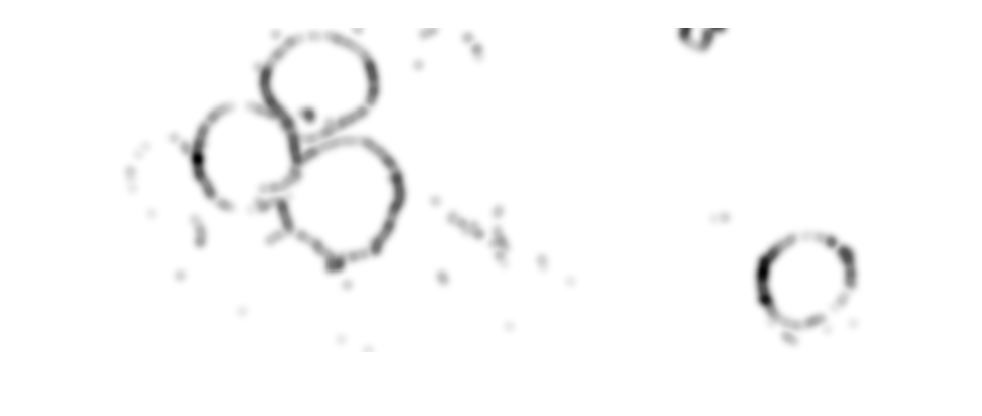
\includegraphics[scale=0.5]{img/Eext.png}
		\caption{External energy result}
		\label{fig:Eextforce}
	\end{center}
\end{figure}

\begin{figure}
	\begin{center}
		\centering
		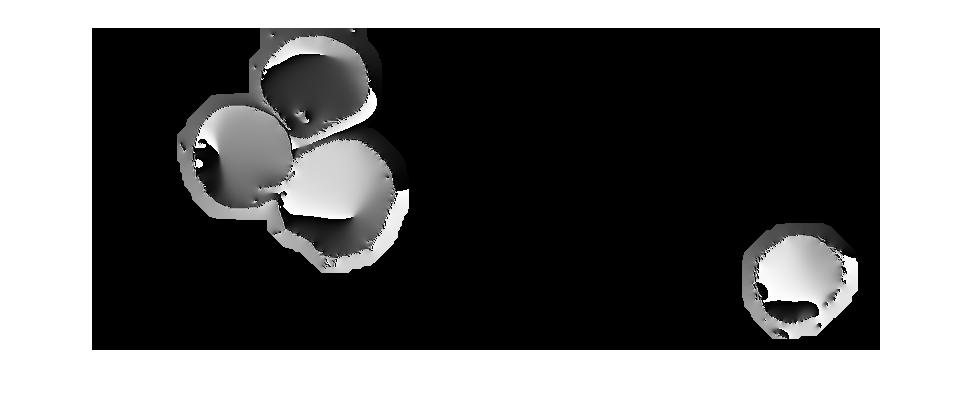
\includegraphics[scale=0.5]{img/onlyleuco.png}
		\caption{image of leukocytes without red blood cells}
		\label{fig:onlyleu}
	\end{center}
\end{figure}
In order to delete all the uniform part of the figure and put in exalt the edges we use a mediand filter using the function $ordfilt2$ searching the 18th element of the $5 * 5$ mask \ref{fig:Pmedonlyleu}.

\begin{figure}
	\begin{center}
		\centering
		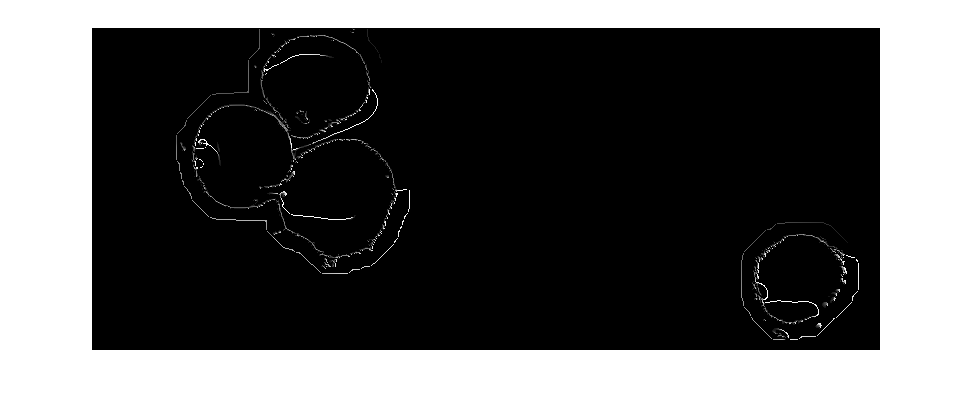
\includegraphics[scale=0.5]{img/Pmedonlyleuko.png}
		\caption{edges and region of leukocytes}
		\label{fig:Pmedonlyleu}
	\end{center}
\end{figure}
\section{Combination of two results: the division method}
The two results that we obtained seems in no-correlation, but the skill of this segmentation lives in this passage. Using the overlay function we search all the points in overlay between the images \ref{fig:Pmedangle} and \ref{fig:Pmedonlyleu}, using the red color to isolate the leukocytes region \ref{fig:over}.
\begin{figure}
	\begin{center}
		\centering
		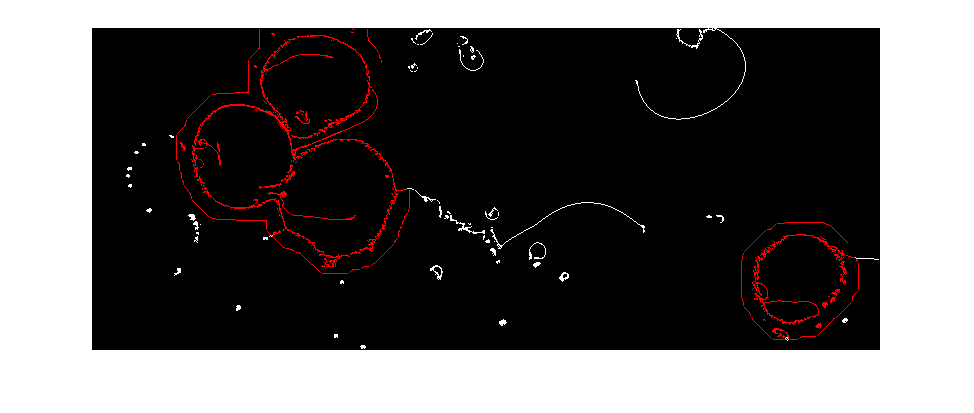
\includegraphics[scale=0.5]{img/overlay.png}
		\caption{overlay of figures \ref{fig:Pmedangle} and \ref{fig:Pmedonlyleu}}
		\label{fig:over}
	\end{center}
\end{figure}
We choose to use the red color, because if we isolating only the red component of the image we can obtain an image that contains only the leukocytes regions. The result of this task is visible in the image \ref{fig:leukoover} 
\begin{figure}
	\begin{center}
		\centering
		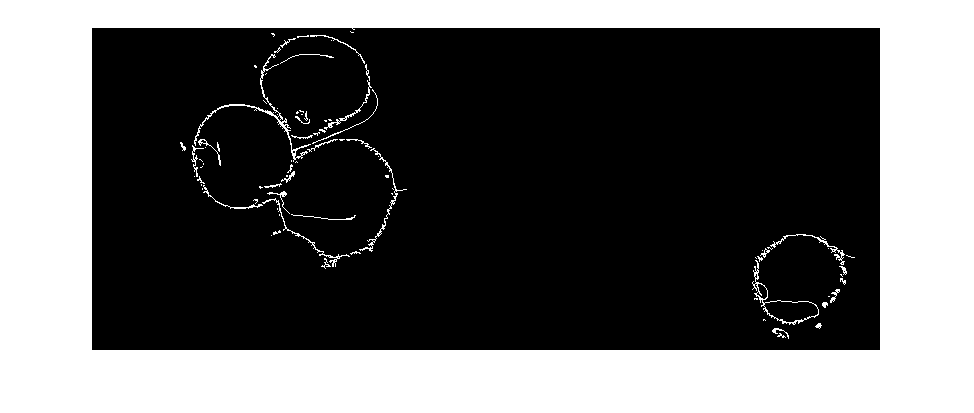
\includegraphics[scale=0.5]{img/overLeuko.png}
		\caption{only leukocytes edges}
		\label{fig:leukoover}
	\end{center}
\end{figure}

\section{Segmentation with the skeleton function}
Starting from the image \ref{fig:leukoover} we have to connect every single white point to the nearest. To do this task we use the function $imdilate$ to dilate all the white dots with a diamond structural element with the size of 6 pixels. after this step we apply the closing of the opening with two disk respectively of the size 3 and 4 pixels. Now we can apply the skeleton function or the thinning of the edges. To do this passage we use the Matlab function $bwmorph$ that it's not the best function to do this but is the faster one. We try another skeleton external function written by N. Howe that is very interesting because has a precision to compute the skeleton of the image that is very impressive, but because the Pc latency we can't use the last one function. After the skeleton application we obtain an image that contains some spurious branches \ref{fig:skel}. 
\begin{figure}
	\begin{center}
		\centering
		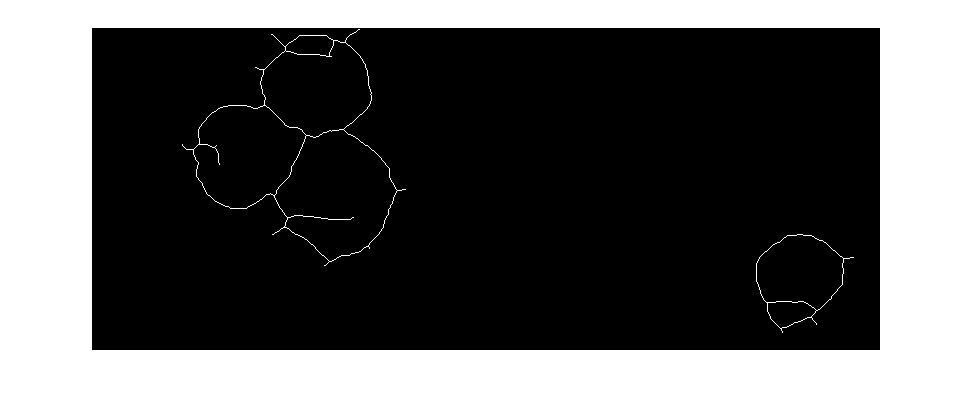
\includegraphics[scale=0.5]{img/skel.png}
		\caption{skeleton of leukocytes with irregular branches}
		\label{fig:skel}
	\end{center}
\end{figure}
To solve this problem is possible to use the Matlab function $bwmorph$ to prune the spurious branches, but in this case the function doesn’t work very well. For this reason we implement a code to resolve the problem. Our code is like a parser that for each point it's see if it is a part of a close circle or not. If it's not a part of a loop the code deletes this point. In a nutshell we save only the point that stay in a 'road' with the starting point and the end point coincident. Below you can read a snippet of pruning code.
\begin{scriptsize}
	\begin{lstlisting} [frame=single]
B = branchpoints;
E = endpoints;
[y,x] = Image;
Dmask = false(size(skel));
	for k = 1:numel(x)
    	D = bwdistgeodesic(skel,x(k),y(k));
    	distanceToBranchPt = min(D(B));
    	Dmask(D < distanceToBranchPt) =true;
	end
skelD = skel - Dmask;
	\end{lstlisting}
\end{scriptsize}

The result that we obtain from the skeleton application is a summary work, indeed we obtain an over-segmentation as is viewable from the image \ref{fig:skelfin}.
\begin{figure}
	\begin{center}
		\centering
		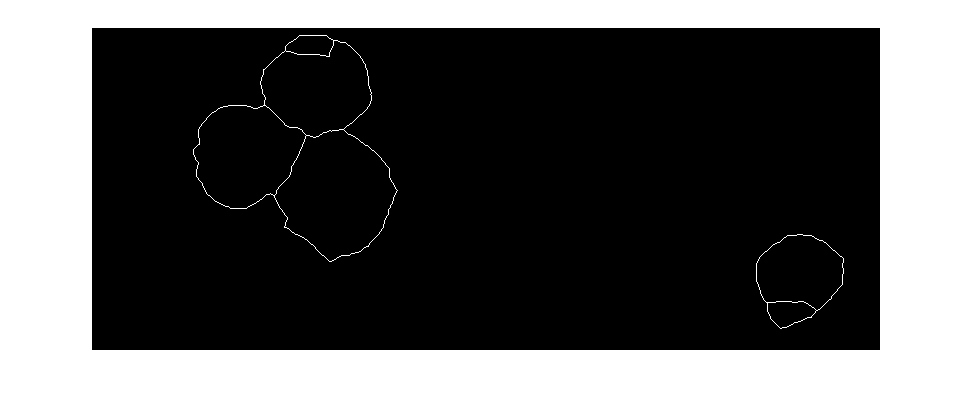
\includegraphics[scale=0.5]{img/skelfin.png}
		\caption{skeleton of leukocytes with no spurious branches}
		\label{fig:skelfin}
	\end{center}
\end{figure}
This over-segmentation isn't good for the correct visualization of leukocytes, but gives us a starting point to improve the solution and to obtain a better result.
Then we try to combine the various result to obtain a segmentation that was similar to the original image. First of all we close all the holes that are inside the image, to obtain a sort of black and white mask. Another fundamental step is sum the skeleton image with the mask. Doing this step we can separate the foreground by the background. Now we can use for the last time the map of edges that we used to calculate the VFC field. We use it summarizing it with the image of leukocytes in foreground and passing this image sum as input to the function $bwareafilt$. We do this because this function extracts all connected components (objects)
from a binary image where the area is in range, producing the segmented image of the leukocytes \ref{fig:bwarea}.
\begin{figure}
	\begin{center}
		\centering
		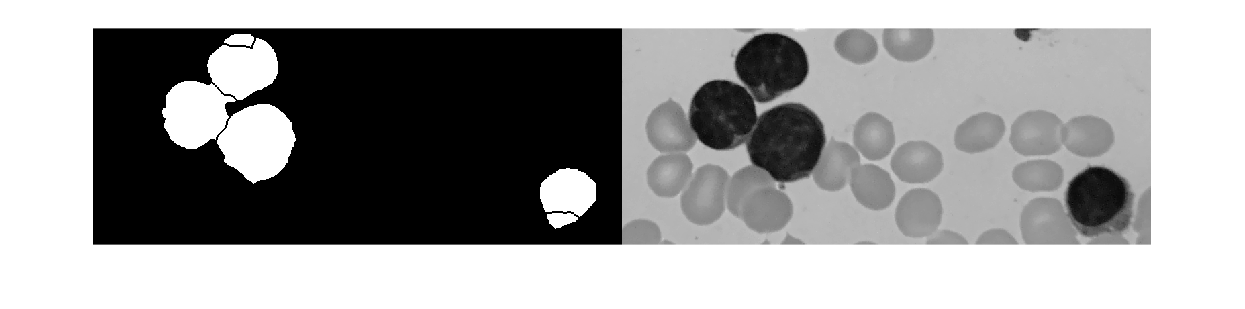
\includegraphics[scale=0.3]{img/segmentation.png}
		\caption{final leukocytes segmentation }
		\label{fig:bwarea}
	\end{center}
\end{figure}
\section{Cells counting}
To understand if all that we did had a sense, we have to do a counting of the cells. Because the images have a low definition we can found an over segmentation inside the cells, but it's easy to overtake this problem without consider the little regions that are inside the image. Then if we delete all the regions that are less than an upperbound we can have the exact number of leukocytes inside the image. We do this using the following snippet code
\begin{scriptsize}
	\begin{lstlisting} [frame=single]
CC = bwconncomp(BW2,8);
numPixels = cellfun(@numel,CC.PixelIdxList);
[~,idx] = min(numPixels);

while min(numPixels)<2000
    BW2(CC.PixelIdxList{idx}) = 0;
    CC = bwconncomp(BW2,8);
    numPixels = cellfun(@numel,CC.PixelIdxList);
    [~,idx] = min(numPixels);
end
[labeledImage, numberOfObject] = bwlabel(BW2);
	\end{lstlisting}
\end{scriptsize}
The resulting image of this consider only the the regions that are the same size of the nucleus or bigger.
\begin{figure}
	\centering
	\begin{subfigure}[b]{0.6\textwidth}
        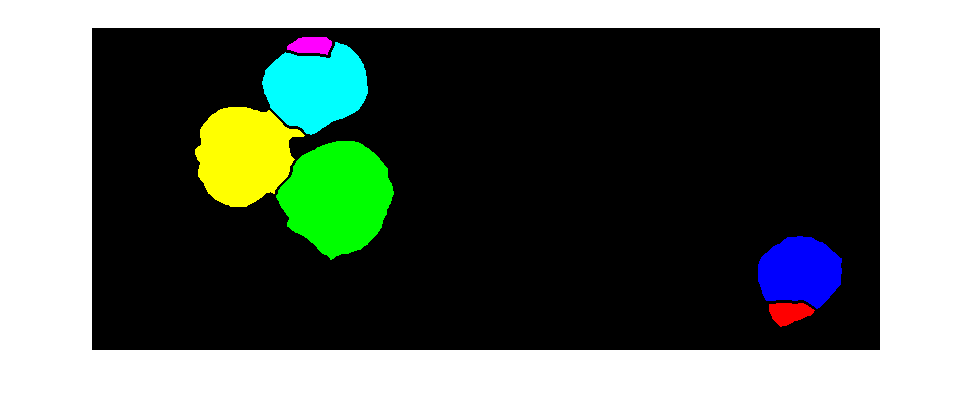
\includegraphics[width=\textwidth]{img/celluleConCito.png}
        \caption{ }
        \label{fig:alltheregions}
    \end{subfigure}
    \begin{subfigure}[b]{0.6\textwidth}
		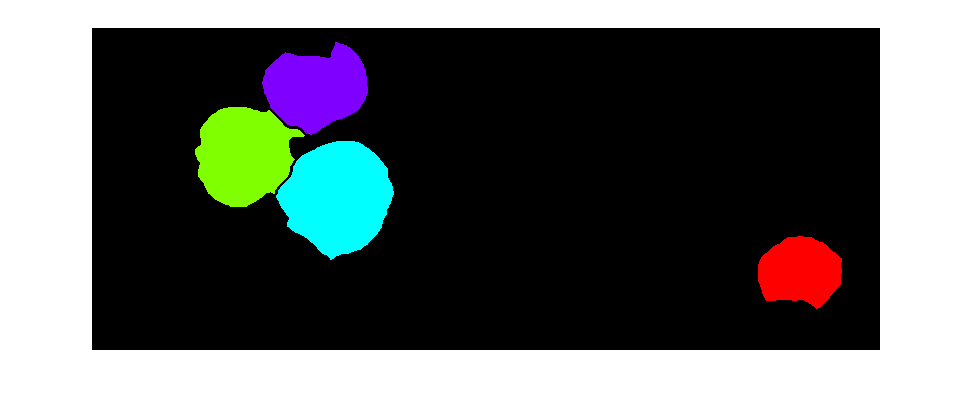
\includegraphics[width=\textwidth]{img/conteggioNuclei(noWatersheed).png}
		\caption{ }
		\label{fig:onlybigregions}
	\end{subfigure}
	\caption{(a) All the regions, (b) Only big regions}
	\label{fig:counting}
\end{figure}
\part{Results and conclusions}
\chapter{Experimental results and conclusions}
\section{Results}
Our propose in a nutshell is a new substitutive method of Watershed transform. The following results are obtained using an Acer Aspire E1 laptop with 8 gb of RAM. The figure \ref{fig:alltheprocess} shows all the process starting from the gray scale image to the mask used to find only the leukocytes.
\begin{figure}[htbp]
    \centering
    \begin{subfigure}[b]{0.45\textwidth}
        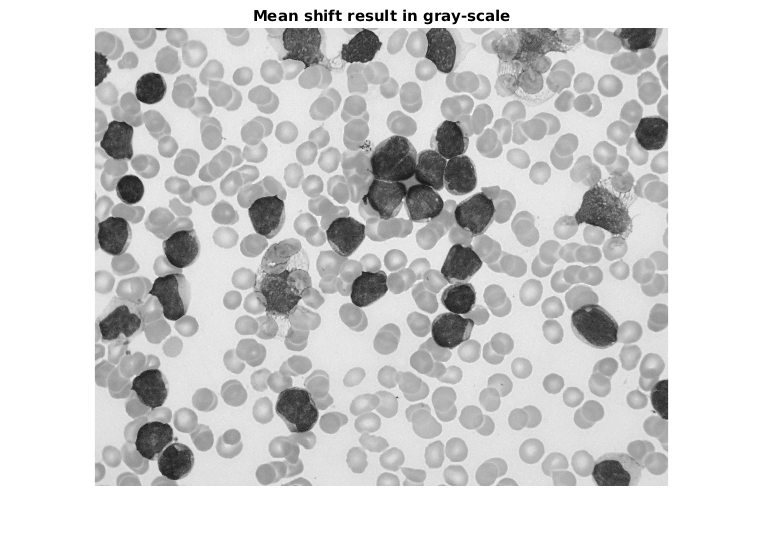
\includegraphics[width=\textwidth]{img/final/figure1.png}
        \caption{ }
        \label{fig:fig1}
    \end{subfigure}
      %(or a blank line to force the subfigure onto a new line)
    \begin{subfigure}[b]{0.45\textwidth}
        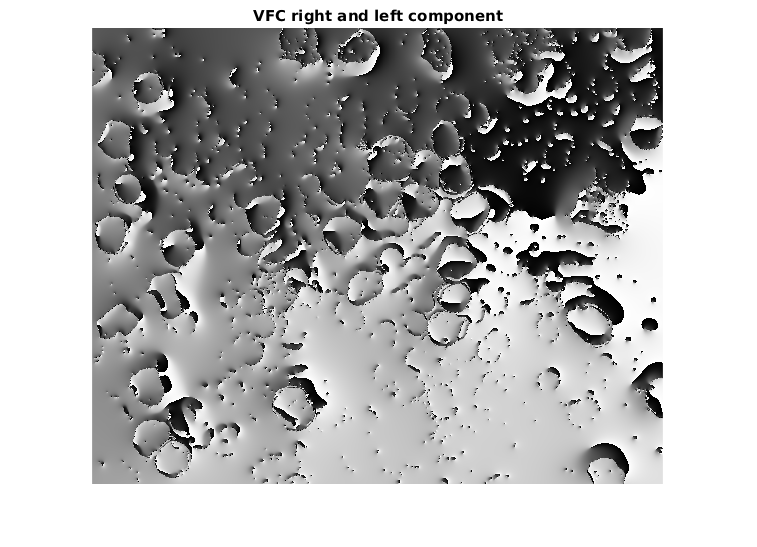
\includegraphics[width=\textwidth]{img/final/figure2.png}
        \caption{ }
        \label{fig:fig}
    \end{subfigure}
    \begin{subfigure}[b]{0.45\textwidth}
        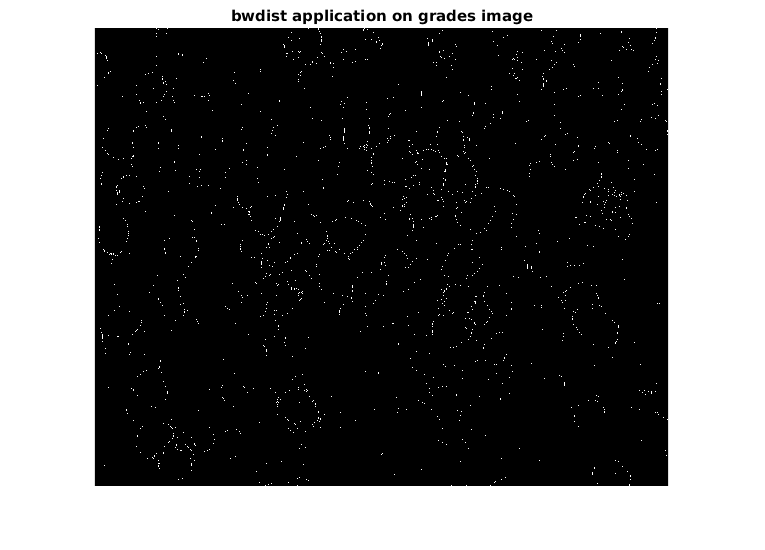
\includegraphics[width=\textwidth]{img/final/figure3.png}
        \caption{ }
        \label{fig:fig3}
    \end{subfigure}
    \begin{subfigure}[b]{0.45\textwidth}
        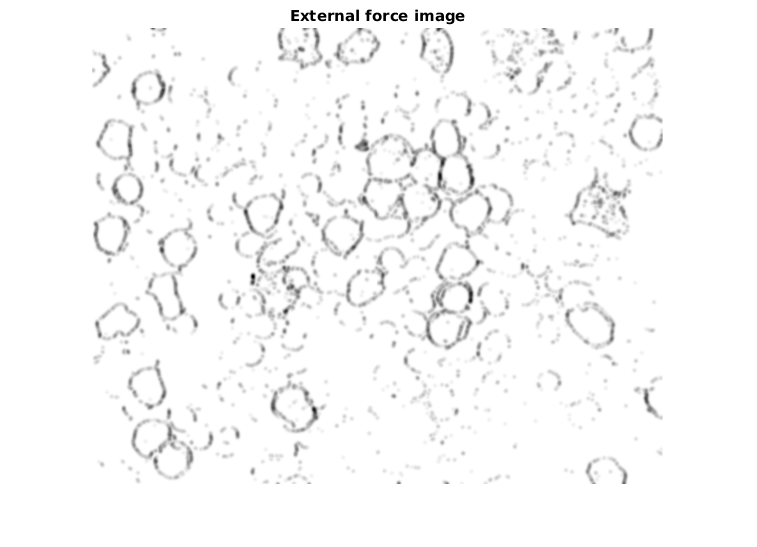
\includegraphics[width=\textwidth]{img/final/figure4.png}
        \caption{ }
        \label{fig:fig4}
    \end{subfigure}
    \begin{subfigure}[b]{0.45\textwidth}
        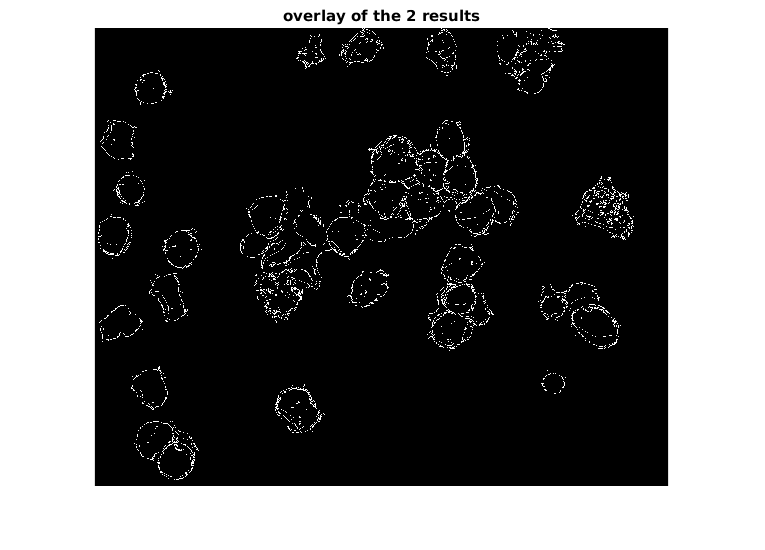
\includegraphics[width=\textwidth]{img/final/figure5.png}
        \caption{ }
        \label{fig:fig5}
    \end{subfigure}
    \begin{subfigure}[b]{0.45\textwidth}
        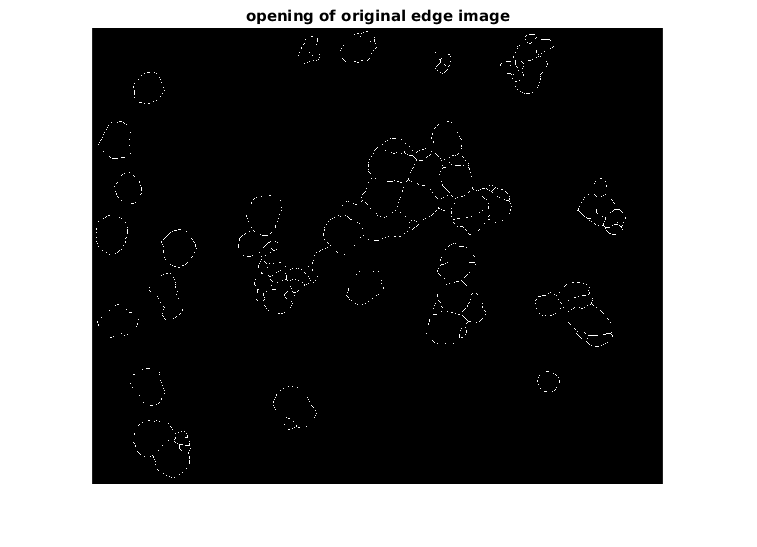
\includegraphics[width=\textwidth]{img/final/figure6.png}
        \caption{ }
        \label{fig:fig6}
    \end{subfigure}
    \begin{subfigure}[b]{0.45\textwidth}
        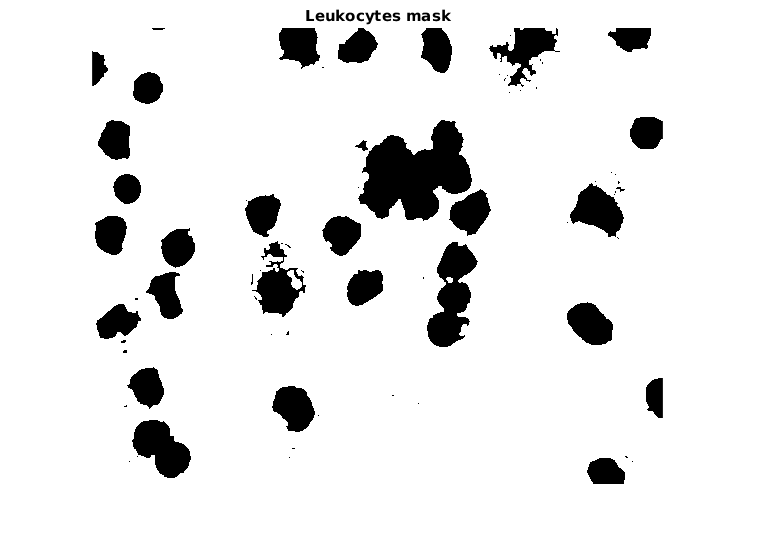
\includegraphics[width=\textwidth]{img/final/figure7.png}
        \caption{ }
        \label{fig:fig7}
    \end{subfigure}

    
    \caption{(a) Mean shift result in gray scale,(b) VFC u and v components,(c) Distance transform on grades image,(d) External force image,(e) Overlay of two results,(f) Opening of initial edge image,(g) Leukocytes mask}
    \label{fig:alltheprocess}
\end{figure}
The last two figures \ref{fig:fig8} \ref{fig:fig9} show the real result of the segmentation.

\begin{figure}
\centering
	\begin{center}
		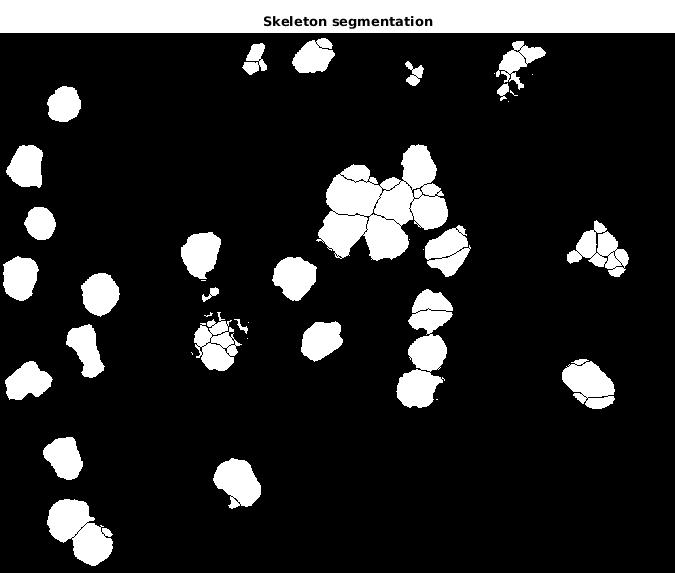
\includegraphics[scale=0.5]{img/final/figure8.png}
		\caption{Skeleton segmentation}
		\label{fig:fig8}
	\end{center}
\end{figure}
\begin{figure}
\centering
	\begin{center}
		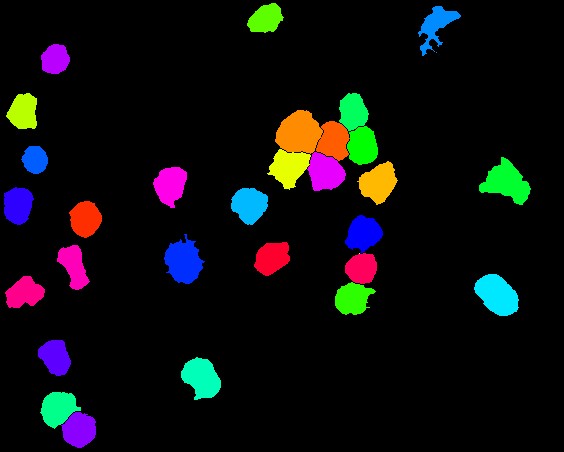
\includegraphics[scale=0.5]{img/final/untitled.png}
		\caption{Merging of little area to count the number of leukocytes}
		\label{fig:fig9}
	\end{center}
\end{figure}
\bigskip
\begin{figure}
\begin{center}
		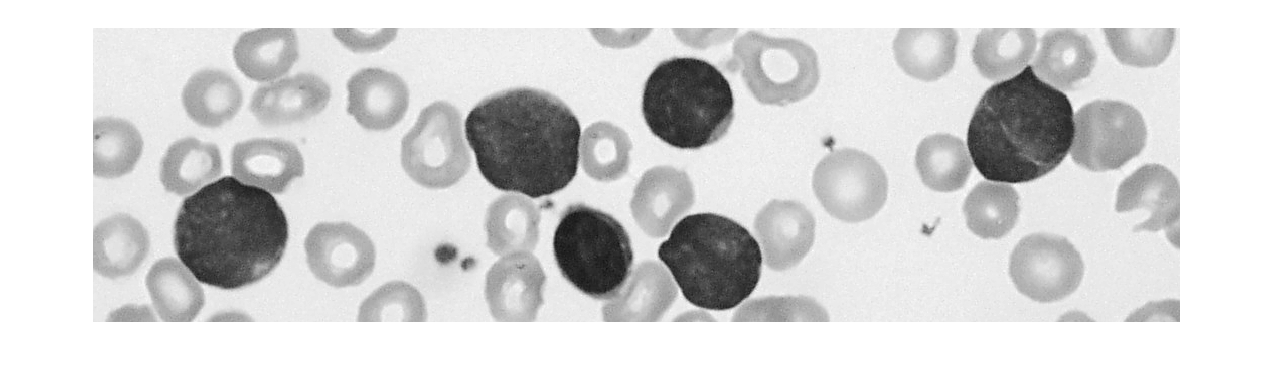
\includegraphics[scale=0.3]{img/final/nooverlap.png}
		\caption{Granulocite after Mean shift application}
		\label{fig:noover}
\end{center}
\end{figure}
\begin{figure}
\begin{center}
		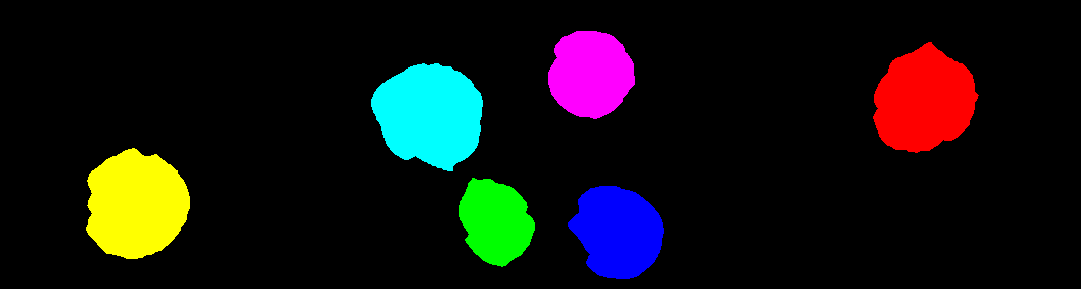
\includegraphics[scale=0.3]{img/final/nooverlapseg.png}
		\caption{Granulocite after Mean shift application}
		\label{fig:nooverseg}
\end{center}
\end{figure}

As it possible to see, between the two images \ref{fig:fig8} and \ref{fig:fig9} there are some differences. The more visible difference is the bigger presence of agglomerate of small areas that create a kind of cell in the first segmentation. This is happened because it was an artefact caused by the Giemsa stain method, but in our approach we can discriminate all this little areas going to remove them because the over-segmentation of this kind (where there are only little areas) means that isn't a leukocyte but only a stain of colour. The result of the counting in this case is 29. 
Working with cropped images we obtain a better result because we have to analyse less cells and as a consequence we have an increase of the speed as is explained in the table \ref{statistics}.
\begin{table}
\centering
\begin{tabular}{|c|c|c|c|}
\hline 
name & cropped & time & Number of recognized cells / number of real cells\\ 
\hline 
image 5 & no & 45.050214 & 29/29\\ 
\hline 
image 5 & yes & 2.214306 & 7/7\\ 
\hline 
image 13 & no & 31.827737 & 11/11 \\ 
\hline 
image 13 & yes & 1.189616 & 4/4 \\ 
\hline 
image 18 & no & 31.493120 & 18/17\\ 
\hline 
image 18 & yes & 1.717642 & 3/3 \\ 
\hline 
\end{tabular} 
\caption{Statistics result}
\label{statistics}
\end{table}
The table shows only the images where is present the worst case of overlap and clump between the cells. The images where is not present any kind of contact between the cells are well segmented with no problem of over-segmentation. In the images  \ref{fig:noover}, \ref{fig:nooverseg} there is an example of segmentation of six cells without any kind of over-segmentation or division. This is only an example but our implementation works very well with all the images with no overlapped cells. In this case is not useful the mean shift application because the cells are well distant from their selves. This means that the computational cost is very less then the version with the mean shift application (total time $<$ 1 second).

\section{Conclusions and future works}
The dissertation proposed an innovative white blood cell recognition and segmentation. It was implemented using some notions already known in literature but never applied in this field. Combining them we obtain a new innovative method in which the major innovation is the use of the Vector field convolution in union to the mean shift and the skeleton function to obtain a result better of the watershed.

\bigskip

The algorithm obtains good results where we analyse images where is not present the granulocyte, because the shape of it's nucleus produce a lot of over-segmentation.\ref{fig:grangray}\ref{fig:gran}
\begin{figure}
\begin{center}
		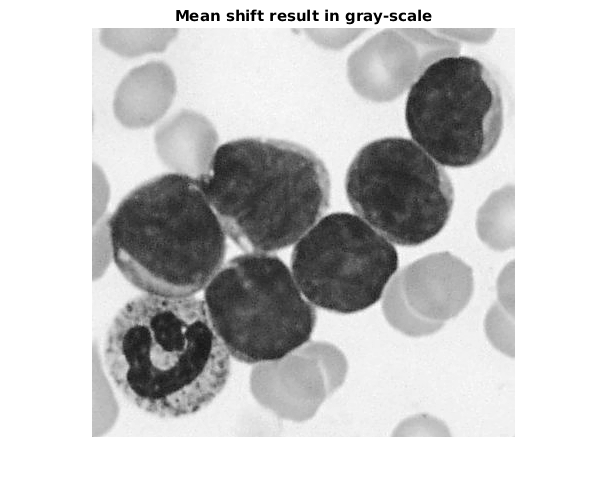
\includegraphics[scale=0.5]{img/final/meangran.png}
		\caption{Granulocite after Mean shift application}
		\label{fig:grangray}
\end{center}
\end{figure}
\begin{figure}
\begin{center}
		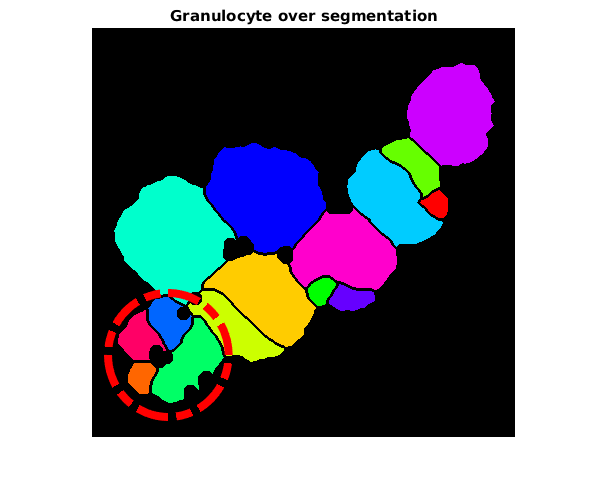
\includegraphics[scale=0.5]{img/final/fingran.png}
		\caption{Over-segmentation caused by the granulocyte}
		\label{fig:gran}
\end{center}
\end{figure}

The most important points that we focused in this thesis can be listed in four sections:
\bigskip

\begin{minipage}{\linewidth}
\begin{enumerate}
\item preprocessing using the mean shift algorithm in order to delete all the differences of colour inside the cells;
\item extrapolation of the right and left component of the VFC force;
\item application of the skeleton in order to separate the overlapped cells;
\item recognize and count of the cells.
\end{enumerate}
\end{minipage}

\bigskip

Our method demonstrates that at this moment is better than everyone algorithm existing in literature. The only problem is the less robustness causing by the low quality images and the over-segmentation caused by the granulocytes. But as the literature says, this is the complex field in histologic image segmentation.

\bigskip

Is possible to resolve this robustness problem. As future works we want to implement a new kind of region merging in order to delete all the over-segmentation caused by the granulocyte and a new points liking function to remove the skeleton side of the algorithm and use only the informations give by the VFC components. 

% ================================================================
% PARTE FINALE
% ================================================================
\backmatter

\listoffigures
\listoftables
%\listoflistings
%\addcontentsline{toc}{chapter}{List of Listings}

\printbibliography[heading=bibintoc]



\end{document}